% ==============================================================================
% TCC - Nome do Aluno
% Capítulo 2 - Referencial Teórico
% ==============================================================================
\chapter{Algoritmos de menor caminho em Grafos estáticos}
\label{sec-algoritmosestaticos}

\section{Algoritmo de Dijkstra}
\label{sec-dijkstra}

\subsection{Definição}
\label{sec-dijkstra-algoritmo}
O algoritmo de Dijkstra foi proposto por Edgar W. Dijkstra em 1959 \cite{dijkstra1959note}. Ele tem por objetivo definir o menor caminho partindo do vértice origem $v_{s}$ e chegando a todos os demais vértices $v_{i}$ do grafo $G = (V,E)$. Para garantir a viabilidade do algoritmo, assume-se que todos os pesos $w( u, v )$ sejam maiores ou iguais a zero para toda aresta $E$ do grafo $G$ \cite{cormen2009introduction}.

A seguir é apresentado o pseudocódigo do algoritmo conforme descrito em \citeonline{drozdek2012data}.
%\begin{verbatim}
%CÓDIGO AQUI
%\end{verbatim}

\begin{lstlisting}[ mathescape, label=lst-dijkstra-codigo, caption=Algoritmo de Dijkstra., float=htpb]
DijkstraAlgorithm(weighted simple digraph, vertex first)
	for all vertices v
		currDist(v) = $\infty$;
	currDist(first) = 0;
	toBeChecked = all vertices;
	while toBeChecked is not empty
		v = a vertex in toBeChecked with minimal currDist(v);
		remove v from toBeChecked;
		for all vertices u adjacent to v and in toBeChecked
			if currDist( u ) > currDist( v ) + weight( edge(vu) )
				currDist( u ) = currDist( v ) + weight( edge(vu) );
				predecessor( u ) = v;
\end{lstlisting}

O algoritmo inicia atribuindo o valor inicial da distância de cada vértice do grafo igual a $\infty$, com exceção do vértice inicial $v_{s}$ que será iniciado por 0. Em seguida todos os vértices são adicionados ao conjunto ``toBeChecked'' (``aSeremChecados''). Feito isso, inicia-se o processo iterativo: seleciona-se o vértice $v$ de menor custo que esteja dentro do conjunto ``toBeChecked'', retira-se ele do conjunto e a partir dele, para cada vértice adjacente $u$ de $v$, é verificado se a distância atual calculada de $u$ é maior do que a distância calculada de $v$, mais o valor referente ao peso da aresta de $v$ a $u$ (origem em $v$). Caso seja verdade, a distância atual de $u$ é substituída pela soma da distância atual de $v$ mais o peso da aresta de $v$ a $u$ (este valor corresponde à distância do vértice de origem $v_{s}$ até $u$), além de definir o antecessor de $u$ como $v$. Repete-se o passo iterativo até que o conjunto ``toBeChecked'' esteja vazio\footnote{Em linguagens de programação, é costume substituir o valor $\infty$ pelo maior número representativo do tipo da variável selecionado para representar a distância. Por exemplo na linguagem C, caso se utilize o valor int (inteiro) para representar a distância, a atribuição inicial será dado pela constante INT\underline{\space}MAX  definida pela biblioteca ``limits.h'', que representa o maior valor numérico representado por esse tipo de variável.}.
\newpage
Ao final do algoritmo, teremos o conjunto de predecessores de cada vértice do grafo, e a partir deste, poderemos definir a rota para qualquer vértice do grafo partindo de $v_{s}$. O caminho retornado é garantidamente ótimo como mostra \citeonline{cormen2009introduction}.

A figura \ref{fig-dijkstra-algoritmo-grafo} mostra um exemplo de aplicação do algoritmo a um grafo.

\begin{figure}[H]
\centering
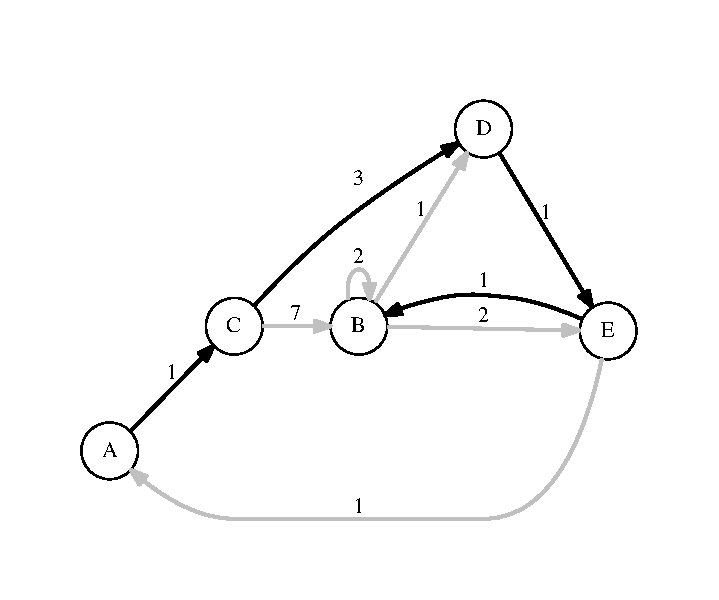
\includegraphics[width=1.\textwidth]{figuras/grafo-dijkstra} 
\caption{Aplicação do algoritmo de Dijkstra tendo o vértice ``A'' como origem. As arestas pintadas de preto correspondem a rota calculada a todos os demais vértices.}
\label{fig-dijkstra-algoritmo-grafo}
\end{figure}

Inicialmente a distância do vértice ``A'' é atribuído como zero enquanto de todos os demais é atribuído como $\infty$. Inicia-se o processo iterativo a partir de ``A'' que explora os seus vértices adjacentes, que neste caso só tem um que é o vértice ``C''. A distância de ``C'' é calculada como o valor da distância de ``A'' mais o peso da aresta ``AC'' (que é igual a 1), e o vértice que é atribuído como antecessor de ``C'' é ``A''. Em seguida é escolhido o vértice cuja a distância seja a menor dentro do conjunto ``toBeChecked'' que neste caso é o próprio ``C''. Do vértice ``C'' explora-se os vértices adjacentes dele: ``D'' e ``B''. Suas respectivas distâncias são atribuídas como a distância de ``C'' mais o peso de suas respectivas arestas (currDist( B ) = 7 + 1; currDist( D ) = 3 + 1), além de atribuir como ``C'' os seus respectivos vértices antecessores. Novamente, escolhe-se o vértice com menor distância em ``toBeChecked'' que neste caso será o D (currDist( D ) = 4 < currDist( C ) = 8 < currDist(E) = "Infinito"). Em ``D'' é explorado seu vértice adjacente ``E'' que é atribuído seu valor currDist( E ) como sendo 5 (3 + 1 + 1) e seu vértice antecessor como ``D''. Busca-se novamente o menor valor dos vértices em ``toBeChecked'' que neste caso será o ``E'' (currDist( E ) = 5 < currDist( B ) = 8). Dele explora-se os seus vértices adjacentes ``B'' e ``A''. O único valor da distância que é alterado é o de ``B'' pois o caminho vindo por ``E'' (A->C->D->E = 1 + 3 + 1 + 1) é menor do que o vindo por ``C''  (A->C->B = 1 + 7). Finalmente, o vértice ``B'' é explorado, mas nenhum de seus vértices adjacentes tem o valor de sua distância alterado pois o menor caminho para eles já foi encontrado.

\subsection{Versões do Algoritmo implementadas e suas Estrutura de Dados}
\label{sec-dijkstra-versoes}
Neste projeto de graduação foram implementadas três versões do algoritmo de Dijkstra usando estruturas de dados diversas.

As versões implementadas são o Dijkstra Canônico (descrito a seguir), Dijkstra Heap Binário (subseção \ref{sec-dijkstra-versoes-heap}) e Dijkstra Heap de Fibonacci (subseção \ref{sec-dijkstra-versoes-fibonacci}), todas baseadas em \citeonline{cormen2009introduction} e \citeonline{drozdek2012data}.

Para a versão Dijkstra Canônico o algoritmo utiliza um vetor para armazenar as distâncias calculadas pelo algoritmo (o indíce dos vértices correspondem ao indíce do vetor em que são armazenados), e a cada passo iterativo (conforme demonstrado pelo algoritmo na seção \ref{sec-dijkstra-algoritmo}), uma busca linear é realizada para determinar o vértice (fora do conjunto ``toBeChecked'') cuja distância é menor dentre todas as outras. A complexidade para esse caso é $O(|V^{2}|)$ \cite{drozdek2012data}.

\subsubsection{Dijkstra Heap Binário}
\label{sec-dijkstra-versoes-heap}
Para esta implementação, será utilizada a estrutura de dados heap binária mínima como fila de prioridade. Heaps binárias podem ser descritas como árvores binárias que possuem as seguintes propriedades \cite{drozdek2012data}:
\begin{enumerate}
 \item O valor de cada nodo não é maior do que os valores guardados em cada um de seus filhos.
 \item A árvore é perfeitamente balanceada, e as folhas no último nível estão todas posicionadas mais a esquerda.
\end{enumerate}

Um exemplo de estrutura Heap Binário representada tanto como árvore como vetor pode ser visualizado nas figuras \ref{fig-dijkstra-heapbinario} e \ref{fig-dijkstra-heapvetor} respectivamente.

\begin{figure}[H]
\centering
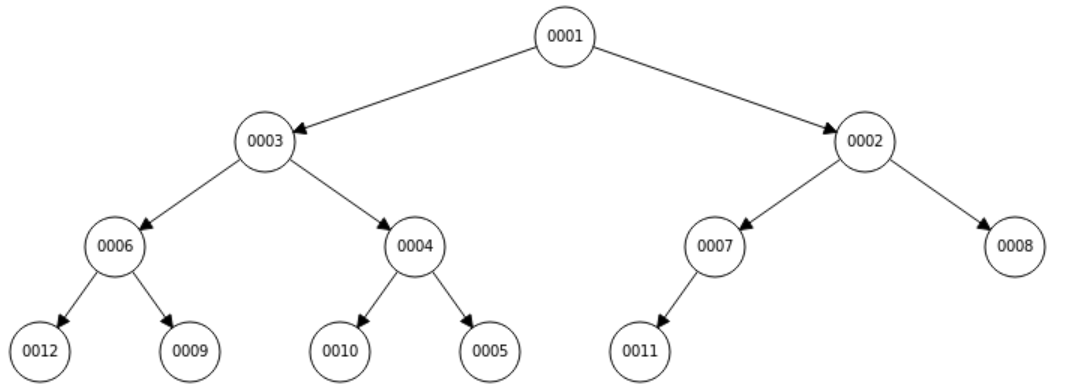
\includegraphics[width=.95\textwidth]{figuras/Heap} 
\caption{Exemplo de Heap Binário representado como árvore.}
\label{fig-dijkstra-heapbinario}
\end{figure}

\begin{figure}[H]
\centering
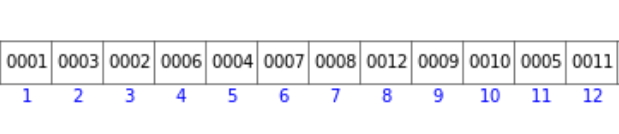
\includegraphics[width=.60\textwidth]{figuras/Heap-vetor}
\caption{Representação do Heap Binário da figura \ref{fig-dijkstra-heapbinario} como vetor.}
\label{fig-dijkstra-heapvetor}
\end{figure}

A disposição dos elementos da árvore no vetor segue as seguintes relações entre nós pai, filho-direita e filho-esquerda:
%\begin{equation}
%Pai(i): \lfloor i/2 \rfloor
%\end{equation}
%\begin{equation}
%Filho-esquerda(i): 2*i
%\end{equation}
%\begin{equation}
%Filho-direita(i): 2*i+1
%\end{equation}
\begin{description}
\item[pai($i$):] $\lfloor i/2 \rfloor$
\item[filho-esquerda($i$):] $2*i$
\item[filho-direita($i$):] $2*i+1$
\end{description}
Sendo que $i \in \mathbb{N}$ e $i \in [1, n]$, em que $i$ representa o índice do elemento no vetor e $n$ o número de elementos da árvore.

 Para efeito de exemplo (observe as figuras \ref{fig-dijkstra-heapbinario} e \ref{fig-dijkstra-heapvetor} para constatação), o nó que está contido na posição 4 do vetor possui como pai o nó de posição 2 ($\lfloor 4 / 2 \rfloor = 2$), tem como filho da esquerda o nó de posição 8 ($2*4 = 8$) e filho da direita o nó de posição 9 ($2*4+1 = 9$).

%\begin{equation}
%\forall i, i \in \mathbb{N} [1,n]
%\end{equation}

A vantagem de se usar essa estrutura de dados reside no fato de suas operações de inserção, extração de mínimo e reconstrução da heap possuírem complexidade de $O(\lg n)$. Com isso, a busca pelo vértice de distância mínima de cada iteração é mais rápida do que a pela realizada pelo Dijkstra Canônico, que para cada escolha do vértice de distância mínima, necessita realizar uma busca linear que é uma operação de custo alto. O tempo computacional utilizando a Heap Binário no algoritmo de Dijkstra é de $O(|E| \lg |V|)$ \cite{cormen2009introduction}.

\subsubsection{Dijkstra Heap de Fibonacci}
\label{sec-dijkstra-versoes-fibonacci}
A Heap de Fibonacci consiste de uma coleção de árvores que seguem a regra de árvore heap mínima, ou seja, os nós pais são maiores ou iguais aos nós filhos. Os nós raízes de cada árvore são interligados por uma lista circular duplamente encadeada. Um ponteiro chamado ``raiz mínima'' aponta para o nó de menor valor.

Sua característica é que operações de adição são executadas de uma maneira ``preguiçosa'', não procurando criar uma forma para as árvores (como por exemplo, deixá-la balanceada), apenas as adicionando à lista principal de raízes. Por consequência, operações de inserção possuem tempo computacional $O(1)$ \cite{cormen2009introduction}. A figura \ref{fig-dijkstra-heapfibonacci1} representa um exemplo da estrutura de Heap de Fibonacci.

\begin{figure}[H]
\centering
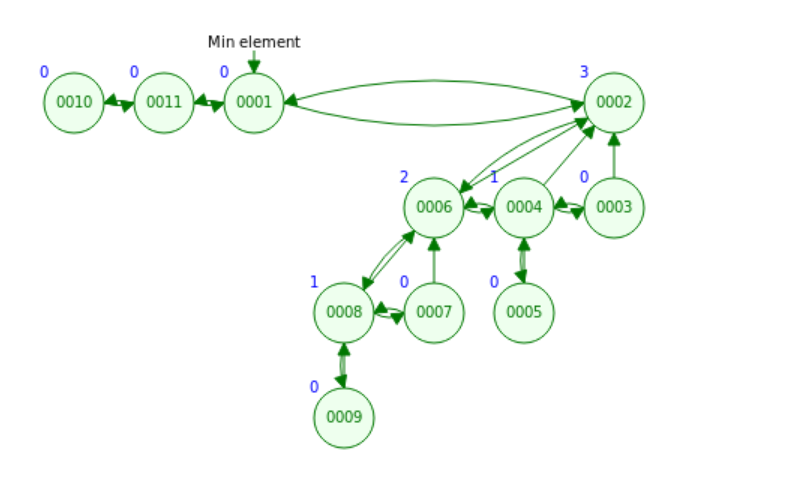
\includegraphics[width=.54\textwidth]{figuras/fibonacci-heap1} 
\caption{Exemplo de Heap de Fibonacci (os números no canto superior esquerdo de cada nodo correspondem ao grau de cada um, ou seja, o número de filhos).}
\label{fig-dijkstra-heapfibonacci1}
\end{figure}

Para operações de extração de mínimo o tempo computacional é mais custoso, devido o fato de que quando o mínimo é retirado, a heap precisa ser reorganizada de forma que sua propriedade principal não seja violada e um novo mínimo seja determinado. Para isso a operação de extração de mínimo se dá em três etapas. Primeiro é retirado o mínimo da heap (caso o mínimo possua nós filhos, eles são colocados na lista principal de raízes) e o seu vizinho é assimilado como o novo mínimo provisório. Em seguida, é preciso definir quem é o novo mínimo e para isso teremos que verificar todos os demais nós raízes. Com o intuito de diminuir o número de nós raízes é que o segundo passo é aplicado.  Ele consiste em agrupar raízes com o mesmo número filhos e para cada par de nodos agrupados, verifica-se qual dos dois é menor. O que for o menor será o nodo pai e outro por consequência será o nodo filho. Após o agrupamento de todos os nodos com mesmo número de filhos, uma busca linear é realizada para se determinar o menor elemento entre os nodos raízes restantes\footnote{Para otimizar a busca de nodos com o mesmo número de grau é utilizado um vetor auxiliar de tamanho mínimo ao maior grau de um nodo da estrutura. Esse vetor contém ponteiros para os nodos e a posição desse nodo no ponteiro corresponde ao grau do nodo. Por exemplo, se um nodo possui grau 3, ele ocupará a posição de número 3 no vetor. Quando um nodo da lista é referenciado na posição que já está ocupado, o processo de lincagem é feito conforme descrito.}. Como exemplo, considere a figura \ref{fig-dijkstra-heapfibonacci1}. Quando o elemento de chave ``0001'' é extraido, o nodo ``mínimo'' é atribuído ao vizinho de ``0001''. Em seguida, é lincado os nodos ``0010'' e ``0011'' por possuírem mesmo número de filhos. É verificado qual dos dois é menor, e que neste caso é ``0010''. Por consequência, este será o nodo pai. O nodo ``0002'' não é lincado com nínguém pois só ele possui 3 filhos. Terminado o processo de lincagem de raízes, uma busca linear é realizada, e o nodo ``0002'' é selecionado como novo nodo mínimo por ser o menor entre os nodos raízes. A figura \ref{fig-dijkstra-heapfibonacci2} mostra a estrutra Heap de Fibonacci da figura \ref{fig-dijkstra-heapfibonacci1} após a operação de extração de mínimo. O tempo computacional para a extração de mínimo é $O(\lg n)$ \cite{cormen2009introduction}.

%\footnote{Para otimizar a busca de nodos com o mesmo número de grau é utilizado um vetor auxiliar de tamanho mínimo ao maior grau de um nodo da estrutura. Esse vetor contém ponteiros para os nodos e a posição desse nodo no ponteiro corresponde ao grau do nodo. Por exemplo, se um nodo possui grau 3, ele ocupará a posição de número 3 no vetor. Quando um nodo da lista é referenciado na posição que já está ocupado, o processo de lincagem é feito conforme descrito.}

\begin{figure}[H]
\centering
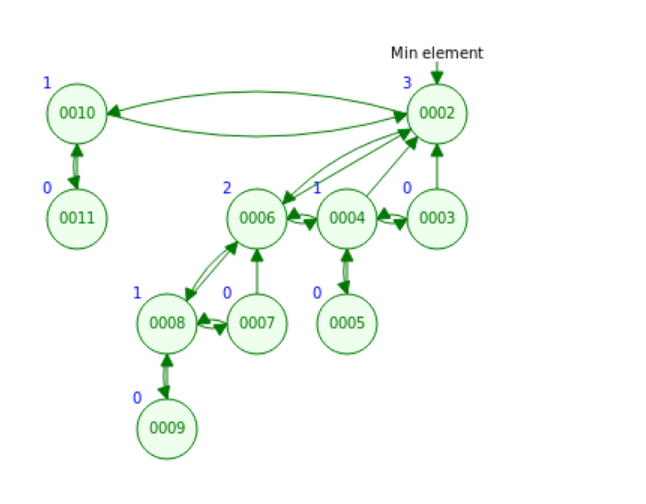
\includegraphics[width=.54\textwidth]{figuras/fibonacci-heap2} 
\caption{Heap de Fibonacci da figura \ref{fig-dijkstra-heapfibonacci1} após a operação de extração de mínimo.}
\label{fig-dijkstra-heapfibonacci2}
\end{figure}


Finalmente para a operação de mudança de chave de um determinado nodo, e após a mudança realizada em tempo constante ($O(1)$), é verificado se a propriedade da heap foi violada. Em caso afirmativo, esse nodo é cortado de seu nodo pai e colocado junto à lista principal. Se o pai não pertencer a lista de nodos raízes, ele é ``marcado'', e caso já estivesse ``marcado'' ele também é cortado e seu pai é ``marcado''. Esse processo continua até encontrarmos um nodo pai ``não marcado'' ou um nodo raiz. No final do processo, verifica-se se o nodo modificado inicialmente é menor do que o nodo mínimo atual. Neste caso, o novo nodo mínimo é o modificado. O tempo computacional é $O(1)$ \cite{cormen2009introduction}.

Por consequência, a complexidade aplicado, neste caso, para o algoritmo de Dijkstra é de $O(|V|\lg |V| + |E|)$ \cite{cormen2009introduction}.

\section{Algoritmo A*}
\label{sec-aestrela}

\subsection{Definição}
\label{sec-aestrela-algoritmo}
O algoritmo A* (lê-se ``A estrela''), também conhecido como busca A*, é um algoritmo de busca informada em grafos. Foi proposta originalmente por \citeonline{hart1968formal} e pode ser visto como uma adaptação do algoritmo de Dijkstra (apresentado no capítulo \ref{sec-dijkstra}) em que, ao invés de se calcular a melhor rota de um ponto de partida para todos os demais vértices do grafo, se estabelece uma boa rota (ou mesmo a rota ótima\footnote{A garantia do valor ótimo do algoritmo depende de fatores que serão discutidos na subseção \ref{sec-aestrela-algoritmo-heuristica}.}) partindo do vértice origem a um vértice destino. Isso é feito realizando ``podas'' do caminho de forma que não seja necessário visitar todos os vértices, apenas os mais promissores do grafo.

A seguir é apresentado o algoritmo A* adaptado de \citeonline{likhachev2008anytime} sobre o algoritmo de Dijkstra apresentado na seção \ref{sec-dijkstra-algoritmo}. 

\begin{lstlisting}[ mathescape, label=lst-aestrela-codigo, caption=Algoritmo A*, float=htpb]
$A^{*}$Algorithm(weighted simple digraph, vertex first, vertex goal)
	for all vertices v
		g(v) = $\infty$;
	g(first) = 0;
	toBeChecked = all vertices;
	while goal is in toBeChecked
		v = a vertex in toBeChecked with minimal f(v);
		remove v from toBeChecked;
		for all vertices u adjacent to v
			if g( u ) > g( v ) + weight( edge(vu) )
				g( u ) = g( v ) + weight( edge(vu) );
				predecessor( u ) = v;
				update u in toBeChecked with f(u) = g(u) + h(u);
\end{lstlisting}

O algoritmo segue em sua essência como um Dijkstra adaptado. Iniciamos a distância de todos os vértices g(v) (valor que corresponde ao valor da distância calculada do vértice origem ``first'' até o vértice ``v'') como sendo $\infty$\footnote{Vide nota de rodapé da seção \ref{sec-dijkstra-algoritmo}.}, com exceção do vértice origem, cujo valor atribuído é zero. Adicionamos todos os vértices ao grupo ``toBeChecked'' \footnote{Algumas literaturas designam esse conjunto como OPEN.}. Feito isso inicia-se o processo iterativo: enquanto o vértice ``goal'' estiver dentro do conjunto ``toBeChecked'' (ou seja, o vértice ``goal'' não foi alcançado ainda), o vértice com menor valor f(v) (que representa a função da chave ordenadora da fila de prioridades) é retirado do conjunto ``toBeChecked'' e para cada vértice adjacente u de v, verifica-se se o valor de g( u ) atual é maior que g( v ) mais o peso da aresta entre v e u (edge(vu)). Em caso afirmativo, o valor de g( u ) é atualizado para g( v ) mais o peso da aresta entre v e u, e v é marcado como o predecessor de u. O valor do peso do vértice u é atualizado na fila de prioridades utilizada (como a heap binária, descrita na subseção \ref{sec-dijkstra-versoes-heap}) com o valor f( u ) = g( u ) + h( u ). O termo h( u ) consiste no valor heurístico que corresponde a uma estimativa da distância de u ao vértice destino ``goal''.

Observe que para o algoritmo A*, diferente do que ocorre em Dijkstra, não se utiliza o valor de g( u ) (valor da distância calculada do vértice origem ``first'' até o vértice ``u'') como chave de ordenamento da fila de prioridade, mas sim esse valor acrescido de h( u ). Observe também que o algoritmo termina ao ser removido o vértice destino (``goal'') da lista do ``toBeChecked'' em contrapartida ao Dijkstra que calcula as distâncias para todos os vértices do grafo. É devido a esse valor que o algoritmo A* realiza ``podas'' no número de vértices a serem checados, buscando os mais promissores, já que esse valor faz com que os vértices cujas estimativas sejam mais próximas do vértice destino (``goal'') sejam colocados mais a frente na fila de prioridades e por consequência, sejam calculados primeiro. E assim é mais provável que o vértice destino seja alcançado antes e tenha sua rota calculada, terminando o algoritmo. O valor h( u ) é classificado como admissível e não-admissível cujo significado será discutido na subseção \ref{sec-aestrela-algoritmo-heuristica}.

A figura \ref{fig-aestrela-algoritmo-mapa1} contida em \citeonline{russell1995modern} mostra um exemplo de aplicação do algoritmo.

\begin{figure}[H]
\centering
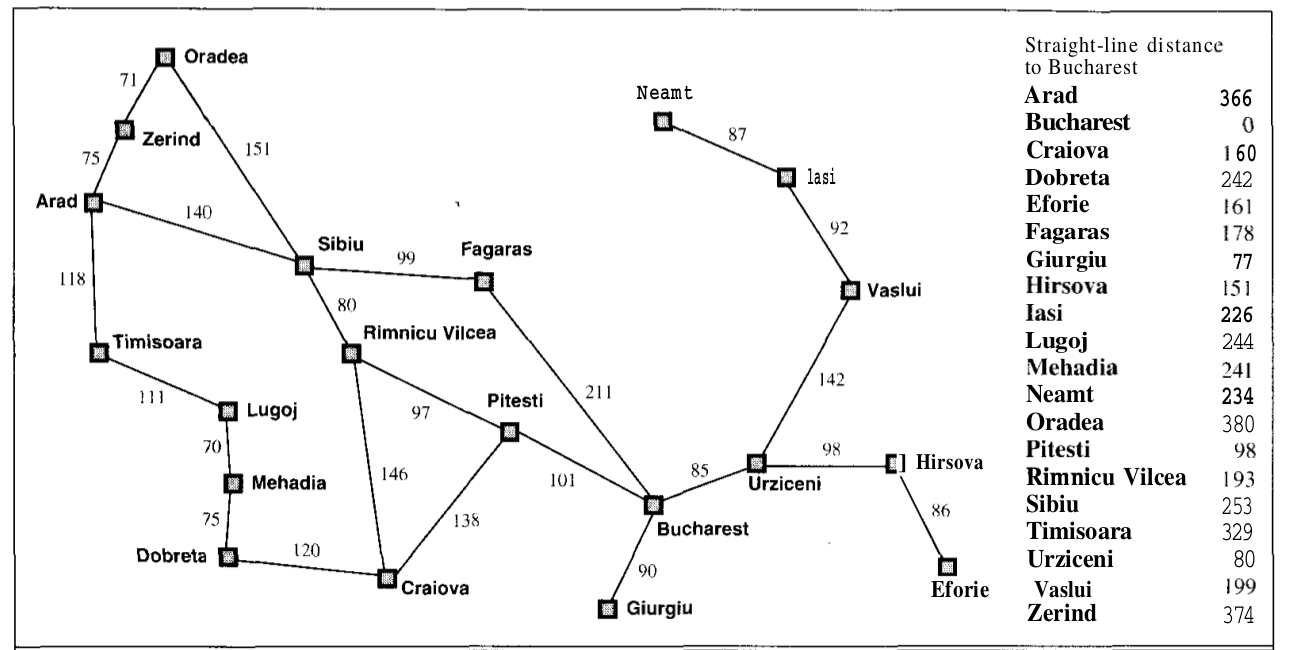
\includegraphics[width=.90\textwidth]{figuras/Aestrela-mapa1} 
\caption{Mapa da Romênia com os valores das distâncias entre as cidades e a distância euclidiana de todas elas até Bucareste.}
\label{fig-aestrela-algoritmo-mapa1}
\end{figure}
\newpage
Um viajante deseja partir da cidade de Arad com destino a Bucareste buscando percorrer o menor caminho entre essas duas cidades. Para isso é utilizado o algoritmo A* que explora o grafo conforme descrito na figura \ref{fig-aestrela-algoritmo-mapa2}\footnote{A figura \ref{fig-aestrela-algoritmo-mapa2} foi obtida do vídeo ``Algoritmo A*'' contido no sítio eletrônico \url{https://www.youtube.com/watch?v=6CqZ5AaTfhQ}, acesso em 25 de abril de 2017.}, tendo como heurística utilizada, a distância euclidiana entre todas as cidades e Bucareste (distâncias também representadas na figura \ref{fig-aestrela-algoritmo-mapa1}).

\begin{figure}[H]
\centering
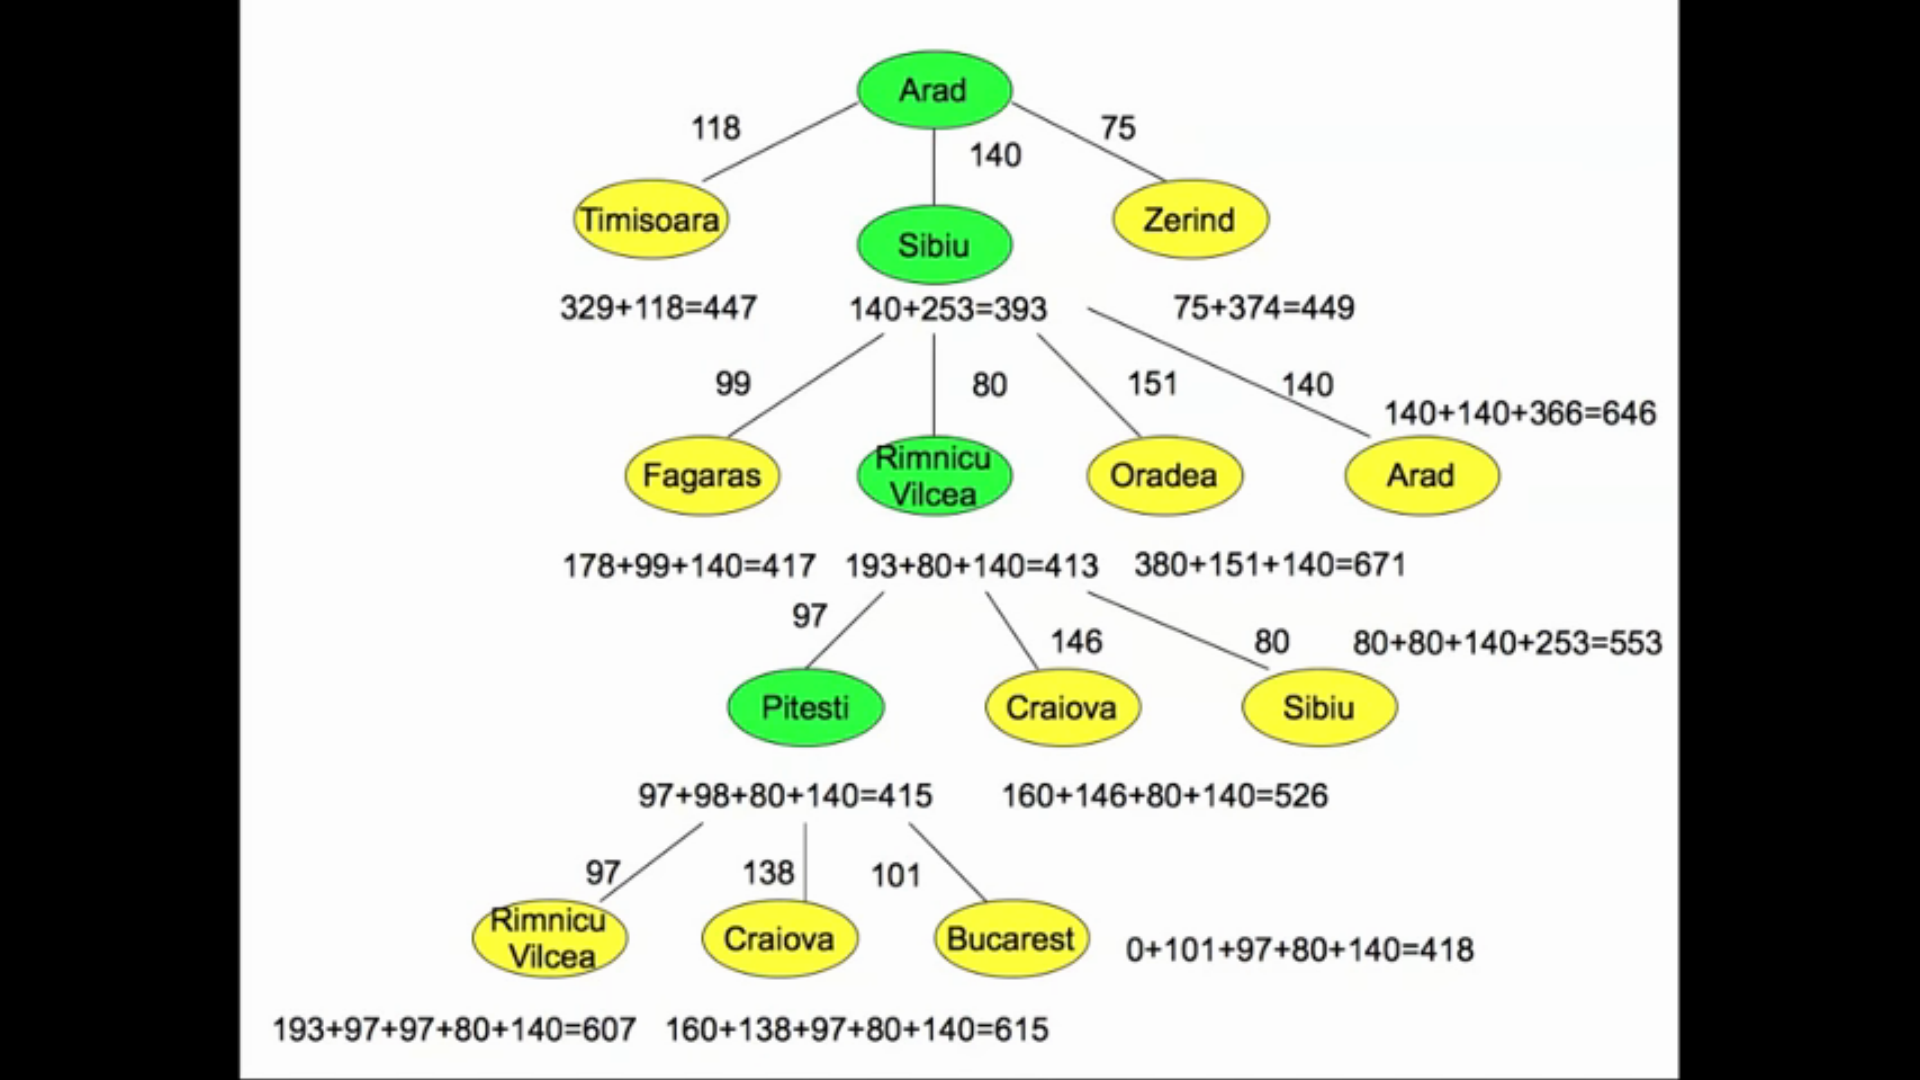
\includegraphics[width=.85\textwidth]{figuras/Aestrela-mapa2} 
\caption{Desenvolvimento do algoritmo A*.}
\label{fig-aestrela-algoritmo-mapa2}
\end{figure}

O procedimento é bem semelhante ao de Dijkstra (descrito no capítulo \ref{sec-dijkstra}). Inicialmente é atribuído o valor de distância de todos os vértices g(v) como $\infty$, com exceção do vértice de origem que é atribuído como zero. Neste exemplo da figura \ref{fig-aestrela-algoritmo-mapa2}, o vértice de origem é a cidade de ``Arad''. Dela se expande para seus vértices vizinhos, que no caso são as cidades de ``Timisoara'', ``Sibiu'' e ``Zerind''. A fila de prioridades é atualizado conforme a função f( u ) = g( u ) + h( u ). Sendo assim o próximo vértice a ser explorado é a cidade de ``Sibiu''. Vemos o fator heurístico ``pesando'' na escolha do próximo vértice a ser escolhido, pois por Dijkstra, o próximo vértice a ser escolhido seria ``Zerind'', ao invés de ``Sibiu'', pois aquela possui aresta com peso menor do que esta. Dela se expande para as cidades vizinhas de ``Fagaras'', ``Rimnicu Vilcea'', ``Oradea'' e ``Arad''. ``Rimnicu Vilcea'' é tida a cidade mais promissora e dela continua a expansão para as suas cidades vizinhas de ``Pitesti'', ``Craiaova'' e ``Sibiu''. ``Pitesti'' é escolhida. E dela se expande para as suas cidades vizinhas de ``Rimnicu Vilcea'', ``Craiova'' e finalmente ``Bucarest'' que é a cidade destino e que tem fator heurístico igual a zero, sendo portanto mais provável a sua escolha na próxima iteração, terminando assim o algoritmo.


%\citeonline{russell1995modern,cormen2009introduction}.

%\begin{lstlisting}[ mathescape, label=lst-aestrela-codigo, caption=Algoritmo A*, float=htpb]
%Entrada: Grafo G, vértice inicial $v_{i}$, vértice destino $v_{f}$
%	para todo vértice $s \in V(G), s \neq vi$ faça
%		$g(s) = \infty$
%	fim para
%	$g(v_{i}) = 0$
%	para todo vértice $s \in V(G)$ faça
%		anterior($s$) = -1
%	fimpara
%	OPEN = {$v_{i}$}
%	enquanto $v_{f}$ não é expandido faça
%		s = desenfila(OPEN)
%		para cada sucessor $s'$ de $s$ faça
%			se $g(s') > g(s) + c(s,s')$ então
%				$g(s') = g(s) + c(s,s')$
%				anterior($s'$) = s
%				insira/atualize $s'$ em OPEN pelo valor de f
%			fim se
%		fim para
%	fim enquanto
%retorna anterior
%\end{lstlisting}



\subsection{Heurísticas admissíveis e não-admissíveis}
\label{sec-aestrela-algoritmo-heuristica}  
O fator heurístico h( u ) é uma estimativa da distância entre o vértice ``u'' e o vértice ``goal''. Ela é chamada de \textbf{admissível} quando o valor da estimativa garantidamente não superestima o valor da distância real entre ``u'' e ``goal'' \cite{russell1995modern}. Um exemplo clássico usado de heurística admissível é a distância euclidiana, já que a menor distância entre dois pontos é uma reta \cite{russell1995modern}.

O cálculo da distância euclidiana porém, nem sempre é a forma mais rápida em termos computacionais, já que geralmente ela é calculada em termos dos pontos geográficos do vértice e esse cálculo envolve exponenciação e radiação. É por isso que existe o uso de heurísticas \textbf{não-admissíveis} que são estimativas que visam a usar cálculos mais simples e que, porém, não há a garantia que essa distância superestime a distância real entre ``u'' e ``goal''. Por consequência não há garantia que o caminho ótimo seja encontrado.

Exemplos de heurísticas não-admissíveis:
\begin{itemize}
\item Distância Manhattan:
\begin{itemize}
\item h( u ) = $| x_{u} - x_{goal} | + | y_{u} - y_{goal}|$;
\end{itemize}
\item Atalho Diagonal:
\begin{itemize}
\item h( u ) = $\sqrt{2} * | y_{u} - y_{goal}| + ( | x_{u} - x_{goal} | - | y_{u} - y_{goal}| )$ [Se a distância $| x_{u} - x_{goal} | > | y_{u} - y_{goal}|$];
\item h( u) = $\sqrt{2} * | x_{u} - x_{goal}| + ( | y_{u} - y_{goal}| - | x_{u} - x_{goal} | )$ [Se a distância $| x_{u} - x_{goal} | < | y_{u} - y_{goal}|$];
\end{itemize}
\end{itemize}